\section{Keyframe-Based Image Captioning}

% We also explore a different approach to video captioning, focusing on keyframe-based image captioning. This method leverages the strengths of image captioning models to generate captions for selected keyframes from videos, rather than processing the entire video sequence.

Beyond the primary video-level architecture, we further investigate a complementary paradigm that treats video captioning as a sequence of keyframe-driven image-captioning tasks. In this variant, keyframes are first distilled from the clip and each is captioned by a image-captioning model, rather than processing the entire video sequence. 


\subsection{Keyframe Selection}

The keyframe selection procedure is designed to minimize redundancy and extract only those frames that represent significant visual changes within the video. This process involves the following steps:

\begin{enumerate}[nosep]
    \item Frame Sampling: Frames are initially sampled from the video at a rate of 1 frame per second (fps). This sampling rate substantially reduces the processing load while maintaining a linear runtime relative to the video duration, which is well-suited for short, single-activity videos typical of the MSVD dataset.
    \item Feature Extraction via Visual Embedding: Each sampled frame is transformed into a high-dimensional feature vector using a Vision Transformer (google/vit-base-patch16-224-in21k~\cite{google-vit-base-patch16-224-in21k}) model pre-trained on the ImageNet-21k dataset. ViT embeddings were selected for their demonstrated robustness to common visual artifacts such as motion blur and variations in illumination, rendering them a reliable foundation for change detection.
    \item Similarity-Based Filtering: A frame is designated as a keyframe if its visual representation is sufficiently dissimilar from that of the preceding keyframe. This determination is made using a cosine similarity metric. A frame is added to the keyframe set if the cosine similarity score between its embedding and that of the last accepted keyframe is below a threshold of 0.95.
\end{enumerate}



\subsection{Image Captioning Model}

\subsubsection{Model Overview}
The image captioning model employs a sophisticated encoder-decoder architecture, integrating a pre-trained Vision Transformer (ViT)~\cite{dosovitskiy2020image} as the encoder and a pre-trained Transformer-based language model (T5)~\cite{google2020t5} as the decoder.

\begin{figure}
  \centering
  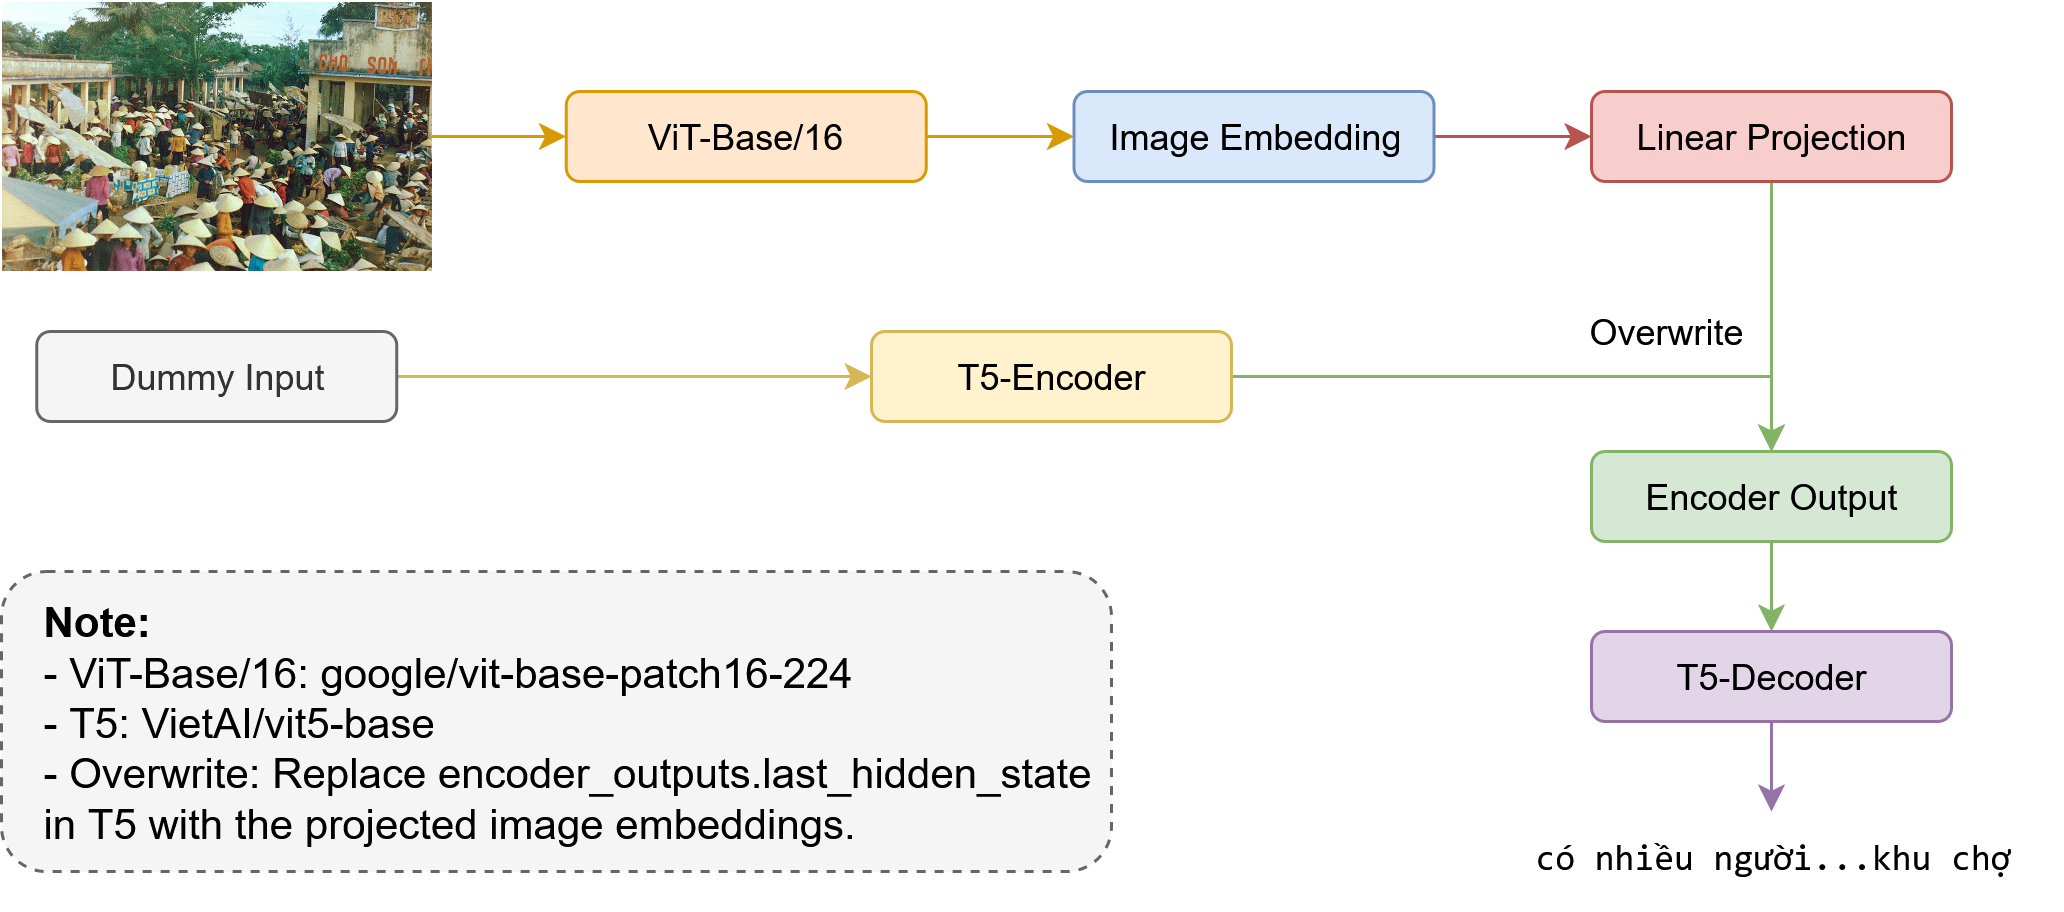
\includegraphics[width=\textwidth]{image/img-captioning-archi.png}
  \caption{The architecture of the ViT-T5 image captioning model, illustrating the integration of the Vision Transformer (ViT) encoder and the T5 decoder.}
  \label{fig:img_cap_archi}
\end{figure}


The visual encoder is a ViT-Base/16~\cite{google-vit-base-patch16-224} model, pre-trained on the ImageNet-21k dataset. Its function is to process an input image and generate a sequence of patch embeddings, which serve as a rich, high-dimensional representation of the image's content.

The text decoder is based on the VietAI/vit5-base~\cite{phan-etal-2022-vit5} model, a T5 variant specifically pre-trained for the Vietnamese language. To bridge the modality gap between the visual encoder and the text decoder, a dedicated interface mechanism was implemented. A linear projection layer maps the embedding dimension of the ViT's output features to the expected hidden dimension ($d_{\text{model}}$) of the T5 decoder.

During the forward pass, the projected visual features directly substitute the output of the T5's own text encoder. Consequently, the T5 decoder's cross-attention mechanism attends directly to this sequence of visual embeddings, enabling it to generate a textual description conditioned on the image content. For generation, the model utilizes a beam search with a beam width of 3 to produce fluent and coherent captions.

\subsubsection{Encoder: Vision Transformer (ViT)}

The choice of the Vision Transformer (ViT) as the encoder was driven by its fundamental architectural advantages over traditional Convolutional Neural Networks (CNNs). Unlike the local receptive fields of CNNs, ViT's self-attention mechanism allows it to capture global context by modeling long-range dependencies between all image patches simultaneously. This holistic understanding of the scene is critical for generating accurate and coherent captions that describe complex interactions between objects. Guided by this motivation, we adopt a pre-trained ViT-Base/16 as our visual encoder.

Concretely, the visual encoder is the backbone of our image captioning model, responsible for transforming a raw image into a sequence of rich feature embeddings that the text decoder can interpret. We employ a pre-trained ViT-Base/16 model, which processes the image as follows (see Figure~\ref{fig:ViT-architecture}):

\begin{itemize}
    \item \textbf{Image Patching:} First, instead of processing pixels individually, the ViT architecture treats an image as a sequence. The input image is divided into a grid of fixed-size, non-overlapping patches. For ViT-Base/16, this means patches of size \(16 \times 16\) pixels.
    
    \item \textbf{Linear Projection of Patches:} Next, each patch is flattened into a one-dimensional vector and linearly projected into a fixed-dimensional embedding space, yielding a sequence of ``patch embeddings''—analogous to word embeddings in NLP.
    
    \item \textbf{Positional Embeddings:} Then, because the Transformer is permutation-invariant, learnable positional embeddings are added to provide spatial context, enabling the model to reason about relative locations of patches.
    
    \item \textbf{Transformer Encoder Layers:} Finally, the resulting sequence is fed into a standard Transformer encoder with:
    \begin{itemize}
        \item \textit{Multi-Head Self-Attention (MHSA):} to weigh relationships among patches (e.g., ``person'' near ``bicycle'').
        \item \textit{Feed-Forward Network (FFN):} a position-wise MLP that further processes each embedding.
    \end{itemize}
\end{itemize}

The encoder outputs a sequence of contextually-aware patch embeddings, which serve as a high-level representation of the image and are subsequently consumed by the T5 decoder to generate the textual description.

\begin{figure}
  \centering
  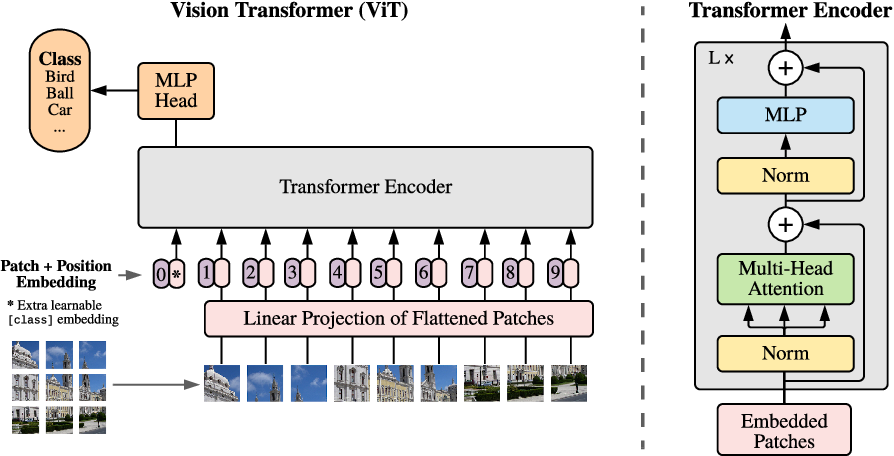
\includegraphics[width=0.85\textwidth]{image/ViT-architecture.png}
  \caption{The architecture of the Vision Transformer model.}
  \label{fig:ViT-architecture}
\end{figure}

\subsubsection{Decoder: T5 Language Model}

The text decoder is the component responsible for generating the final descriptive sentence. For this role, we select VietAI/vit5-base~\cite{phan-etal-2022-vit5}, a T5 variant pre-trained on a large corpus of Vietnamese text. This choice leverages its strong modeling of Vietnamese grammar, syntax, and semantics to produce fluent and natural captions.

While a standard T5 model comprises both an encoder and a decoder, our architecture exclusively utilizes the decoder for text generation. The core challenge is bridging the modality gap so that the text-based T5 decoder can condition on the visual features produced by the ViT encoder. To this end, we replace T5's text encoder with the ViT-derived features via the following steps:

\begin{enumerate}
    \item \textbf{Dimension alignment via linear projection.} Let the ViT patch embeddings have dimension \(d_{\mathrm{ViT}}\) (for ViT-Base/16, \(d_{\mathrm{ViT}}{=}768\)). The T5 decoder expects inputs of hidden size \(d_{\mathrm{model}}\) (for \texttt{vit5-base}, \(d_{\mathrm{model}}{=}768\)). We pass the ViT outputs through a learnable linear layer \(W \in \mathbb{R}^{d_{\mathrm{ViT}} \times d_{\mathrm{model}}}\) to map visual features into the T5 latent space with minimal information loss.
    
    \item \textbf{Encoder-output substitution.} Instead of using T5’s original text encoder, the projected visual features are used to \emph{overwrite} the encoder outputs. Concretely, we construct an encoder output object whose \texttt{last\_hidden\_state} equals the sequence of projected patch embeddings \(\mathbf{H} \in \mathbb{R}^{N \times d_{\mathrm{model}}}\), where \(N\) is the number of visual tokens.
    
    \item \textbf{Cross-attention over visual features.} The T5 decoder employs cross-attention at each generation step to attend to the encoder outputs. By substituting the encoder outputs with \(\mathbf{H}\), the decoder directly attends to the image’s visual representation, enabling token generation to be conditioned on salient regions of the image.
\end{enumerate}

This integration combines the ViT’s strong visual representations with T5’s robust text generation, yielding an effective image-captioning pipeline in Vietnamese.



\begin{figure}[H]
  \centering
  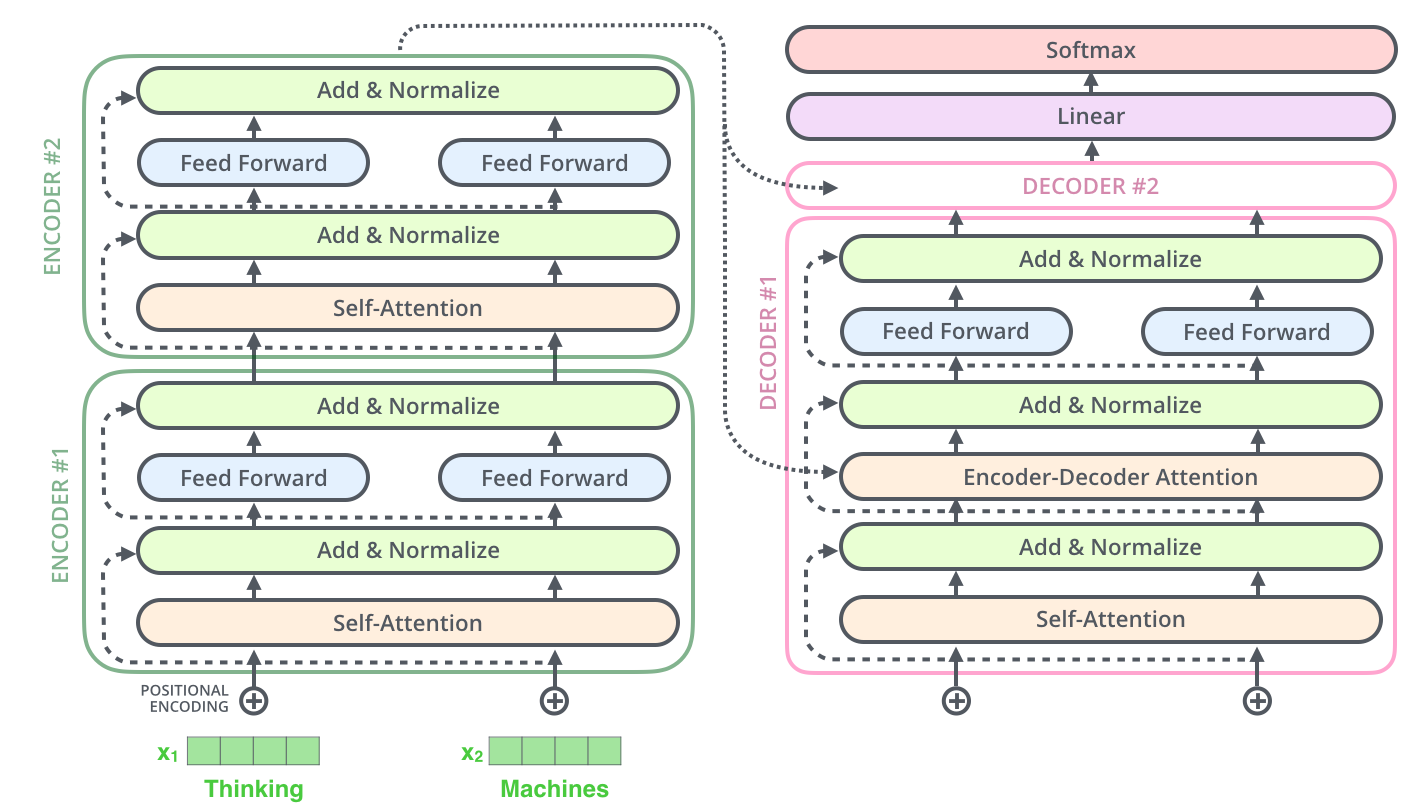
\includegraphics[width=\textwidth]{image/transformer_residual_layer_norm_3.png}
  \caption{The architecture of the T5 model.}
  \label{fig:T5-architecture}
\end{figure}


\subsubsection{Training Procedure}
The model was trained using a parameter-efficient fine-tuning (PEFT) strategy to leverage the knowledge from the pre-trained components while minimizing computational cost and the risk of catastrophic forgetting. During this phase, the weights of the entire ViT encoder and the T5 text encoder were frozen and did not receive updates. Only the parameters of the T5 decoder, the final language model head, and the intermediary linear projection layer were made trainable.

The model was optimized by minimizing the standard cross-entropy loss between the predicted token sequence and the ground-truth captions. We employed the AdamW optimizer with an initial learning rate of $5 \times 10^{-5}$ and a weight decay of $1 \times 10^{-4}$. The learning rate was dynamically adjusted throughout training using a Cosine Annealing schedule with warm restarts.

Training was conducted for a maximum of 8 epochs. To prevent overfitting and select the best-performing model, an early stopping criterion was implemented. This mechanism monitored the validation loss at the end of each epoch and terminated the training process if no improvement was observed for 5 consecutive epochs. The model checkpoint that achieved the lowest validation loss was saved and used for all subsequent evaluations and inference tasks.